\documentclass[10pt,a4paper,twoside,twocolumn]{article}%ustalasz jaki typ dokumentu i właściwości

\usepackage[polish]{babel} % ustawianie języka polskiego
\usepackage[colorlinks=false,linkcolor=green,urlcolor=green,citecolor=green]{hyperref}%hiperłącza ogólnego rodzaju
\hypersetup{pdftitle=Sprawozdanie SSR}

\usepackage{pdfpages} % importowanie plików z pdfa
\usepackage{amsmath} % do wstawiania macierz itp
\usepackage{graphicx} % wstawianie zdjęć
% \usepackage[utf8]{inputenc} % niepotrzebne bo lualatex
\usepackage[T1]{fontenc} % niepotrzebne bo lualatex
\usepackage[left=1cm,right=1cm,top=1cm,bottom=2cm,
columnsep=1cm % odstęp między kolumnami
]{geometry}%marginesy

\usepackage{listings} % punktowanie
% \usepackage{indentfirst} % dawanie akapitu na początku
\usepackage{caption} % podpisy
\usepackage{siunitx} % jednostki si
\usepackage{minted} % ładne kody naprzyklad matlaba
\setminted{linenos=true,frame=single,breaklines=true,breaksymbolleft=,style=vs}

\usepackage{textcase}

\usepackage[polish,nameinlink]{cleveref} % dobre prefiksy przed etykietą i język
\usepackage{cprotect}

\usepackage{fontspec}
% \setmainfont[Ligatures=TeX]{Georgia}
% \setsansfont[Ligatures=TeX]{Arial}
\usepackage{parskip} % usunięcie tab na początku akapitu
\usepackage{newfloat} % aby można było ładnie wstawić elementy typu zdjecie, kod itp

%%% rysowanie wykresów %%% ale w ciul to trudne więc app.diagrams.net
\usepackage{tikz}
\usetikzlibrary{shapes.geometric, arrows, positioning}

% % % SVG import
\usepackage{svg}
\usepackage{import}
\usepackage{xifthen}
\usepackage{transparent}

% \usepackage{mdframed} % ramki
\usepackage[framemethod=TikZ]{mdframed}
\mdfsetup{%
middlelinecolor=red,
middlelinewidth=1pt,
   backgroundcolor=gray!20,
   roundcorner=10pt}

\usepackage{enumitem} % podpunkty customowe

\usepackage{pgfplots}[compat=1.18] % wykresy
%%%%%%%%%%%%%% koniec pakietów %%%%%%%%%%%%%%%%%%%%%%%%%%%



\title{Fajny ten tytuł}%tytuł
\date{\today}%%data
\author{Janusz Chmaruk}%autor
\setcounter{secnumdepth}{3}%głębokość liczenia roździałów

% PRZYKŁAD LICZNIKA ZADAŃ
\newcounter{zadanie}
\newenvironment{zadanie}[1]{
   \refstepcounter{zadanie}
   \subsection*{Zadanie \thezadanie#1}
   \addcontentsline{toc}{subsection}{Zadanie \thezadanie#1} % dodanie do spisu treści
}{}


% DŁUGIE LISTINGI
\newenvironment{longlisting}{\captionsetup{type=listing}}{}

%%%%%%%%%%%%%%%%%%%%%%%%%%%%%%%%%%%%%%%%%%%%%%%%%%%%%%%%%%%%%%%
%%%%%%%%%%%%%%%%%%%%%%%%%%%%%%%%%%%%%%%%%%%%%%%%%%%%%%%%%%%%%%%
%%%%%%% TU SIE ZACZYNA PISANIE PLIKU %%%%%%%%%%%%%%%%%%%%%%%%%%
%%%%%%%%%%%%%%%%%%%%%%%%%%%%%%%%%%%%%%%%%%%%%%%%%%%%%%%%%%%%%%%
%%%%%%%%%%%%%%%%%%%%%%%%%%%%%%%%%%%%%%%%%%%%%%%%%%%%%%%%%%%%%%%

\begin{document}%zaczyna się dokument

% \null%
% 
\includepdf[pages={1}]{Szablon_Projektu.pdf}
\clearpage%następna strona ogółem

\tableofcontents%spis treści
% \clearpage


\begin{zadanie}{}
    Omówić zasadę doboru częstotliwości próbkowania; Zilustrować na przykładzie sygnału $t=0:1$; $y=sin(2*\pi*3*t)$;
    narysuj sygnał i widmo sygnału po spróbkowaniu. \textbf{4p}
\end{zadanie}\\

    \begin{mdframed}[backgroundcolor=gray!20,]
        Częstość próbkowania musi być większa niż dwukrotność częstotliwości najwyższej składowej sygnału.
        $$f_{max} = 3$$
        $$f_{\text{próbkowania}} > 2*f_{max}$$
        $$f_{\text{próbkowania}} > 6$$

        \begin{tikzpicture}
            \centering
            \begin{axis}[
                xlabel={$t$},
                ylabel={$y$},
                xmin=0, xmax=1,
                ymin=-1, ymax=1,
                xtick={0,0.1,0.2,...,1}, % Ustalanie kroków próbkowania
                domain=0:1,
                samples=100
            ]
            \addplot[blue] {sin(deg(6*x))};
            \addplot[red, only marks, mark=*, mark size=1.5pt, samples at={0,0.1,0.2,...,1}] {sin(deg(6*x))};
            \end{axis}
        \end{tikzpicture}
    \end{mdframed}

\begin{zadanie}{}
    Dla filtra o następującej strukturze:
    \begin{figure}[H]
        \centering
        \includegraphics[width=1\linewidth]{Diagram bez tytułu.drawio.pdf}
    \end{figure}
    \begin{enumerate}[label=\alph*)]
        \item podać rodzaj(SOI/NOI) i rząd filtra; \textbf{1p}
        \item wyznaczyć odpowiedź impulsową; \textbf{1p}
        \item narysować odpowiedź na sygnał: $x(k) = \delta (k-1)-\delta(k −3)$; \textbf{4p}
        \item wyznaczyć równanie różnicowe opisujące filtr; \textbf{2p}
        \item wyznaczyć transmitancję filtra; wyznaczyć charakterystykę częstotliwościową filtra; \textbf{2p}
        \item określić stabilność filtra; \textbf{1p}
    \end{enumerate}
\end{zadanie}

\begin{mdframed}[backgroundcolor=gray!20,roundcorner=7pt]
    \begin{enumerate}[label=\alph*)]
        \item Filtr jest SOI, rząd filtra to 3. (CHYBA)
        \item odpowiedź impulsowa to: $h(k) = \delta(2) + (-1)*\delta(k-1) + 3*\delta(k-3)$ (CHYBA, NIE WIEM)
        \item Odpowiedź sygnału:
            \begin{table}[H]
                \centering
                \begin{tabular}{|c|c|}
                    \hline
                    k & y(k) \\ \hline
                    0 & 0 \\ \hline
                    1 & 2 \\ \hline
                    2 & -1 \\ \hline
                    3 & 2 \\ \hline
                    4 & 2 \\ \hline
                    5 & 0 \\ \hline
                    6 & 3 \\ \hline
                    7 & 0 \\ \hline
                \end{tabular}
            \end{table}
        \item Równanie różnicowe:
            $$y(k) = x(k) + 2x(k-1) - x(k-2) + 3x(k-3)$$ (to jest źle, COPILOT)
        \item Transmitacja filtra:$$$$
            Charakterystyka częstotliwościowa filtra:$$$$
        \item Filtr jest stabilny
    \end{enumerate}
    
    
\end{mdframed}



\begin{zadanie}{}
    Na przykładzie filtru dolnoprzepustowego omówić podstawowe cechy ciągłego filtru Czebyszewa. Porównać charakterystyki częstotliwościowe filtru analogowego i cyfrowego. \textbf{3p}
\end{zadanie}

\begin{mdframed}[backgroundcolor=gray!20,]
    
    Charakterystyka amplitudowa flitru jest równomiernie zafalowana w paśmie przepustowym oraz
monotoniczna w zaporowym lub charakterystyka amplitudowa monotoniczna w paśmie
przepustowym oraz równomiernie zafalowana w zaporowym.\\

Filtr Czebyszewa zwykle ma niższy stopień niż filtr Butterwortha przy tych samych
wymaganiach (dzięki bardziej stromej charakterystyce w paśmie przejściowym).\\

(NIE WIEM CZY TO JEST DOBRZE)\\
Porównanie:
\begin{itemize}
    \item Porównując filtry analogowe i cyfrowe, istnieją pewne kluczowe różnice:

    \item Dokładność: Filtry cyfrowe mogą być bardziej dokładne niż ich odpowiedniki analogowe, ponieważ nie są podatne na wpływ szumów i zakłóceń analogowych.
    
    \item Złożoność realizacji: Filtry cyfrowe mogą być trudniejsze do zrealizowania w praktyce, ponieważ wymagają skomplikowanych układów cyfrowych i procesorów sygnałowych.
    
    \item Zakres częstotliwości: Filtry analogowe mogą pracować z sygnałami o wyższych częstotliwościach niż filtry cyfrowe, które są ograniczone przez częstotliwość próbkowania.
    
    \item Zastosowania: Filtry analogowe są często stosowane w radiotechnice i innych aplikacjach, które wymagają przetwarzania sygnałów w czasie rzeczywistym. Filtry cyfrowe są często stosowane w aplikacjach, które wymagają wysokiej dokładności i elastyczności, takich jak przetwarzanie obrazów i dźwięku.
\end{itemize}

    
\end{mdframed}

\begin{zadanie}{}
    Podać warunek liniowej fazy filtrów SOI dla N parzystego i nieparzystego i omówić jaki wpływ ma liniowa faza na filtrowany sygnał? \textbf{3p}
\end{zadanie}

\begin{zadanie}{}
    Podać definicje funkcji autokorelacji R, funkcji autokowariancji C ergodycznego \textbf{1p}, stacjonarnego szeregu losowego X. Wyznaczyć wartość średnią tego procesu oraz funkcję autokorelacji z dostępnej realizacji czasowej $x = [3,5,2,4,2]$ tego procesu losowego. Narysować tę funkcję autokorelacji. \textbf{3p}
    Wyznaczyć macierz autokorelacji R. \textbf{2p}
\end{zadanie}


\begin{zadanie}{}
Filtr Wienera zazwyczaj jest filtrem SOI i pracuje w strukturze


    $$y(n)=\sum_{k=0}^{M}h(k)x(n-k)=h^{T}x(n)$$
    $$h=[h_0,h_1,...,h_M]^{T}$$
    $$x(n)=[x(n),x(n-1),x(n-2)\dots,x(n-M)]^T$$

    \begin{figure}[H]
        \centering
        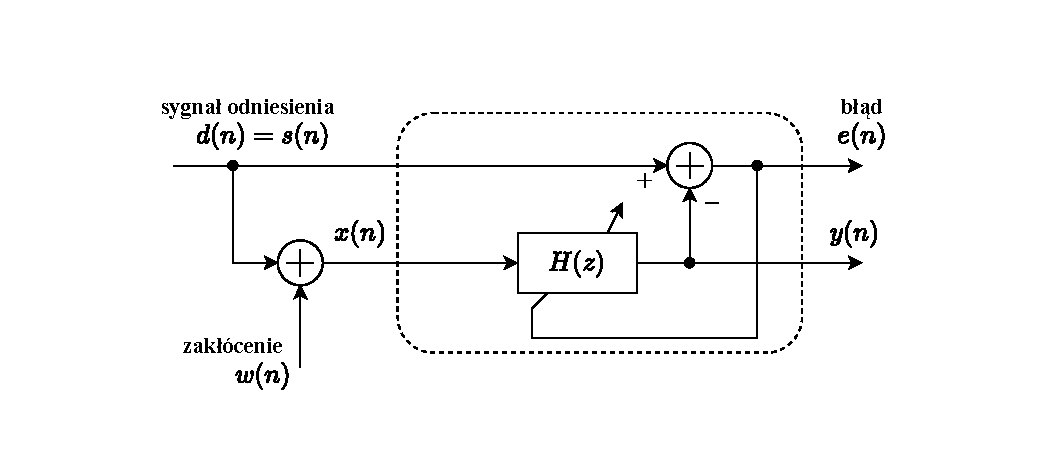
\includegraphics[width=1\linewidth]{2.drawio.pdf}
    \end{figure}
Podać wskaźnik jakości optymalizacji, który prowadzi do uzyskania optymalnego zbioru współczynników filtru \textbf{h}. Podać rozwiązanie problemu optymalizacji w postaci macierzowo-wektorowego równania Wienera-Hopfa. \textbf{4p}
\end{zadanie}




\end{document}